\chapter{Methods}

\startcontents[chapters]
\printmyminitoc{
}


\section{Overview of the method used}



The below diagram shows the overall architecture of the system. We want to try to benefit the representation of the language model in this use case of finding the topics in the corpus of the company's call center.

\begin{figure}[H]
    \centering
    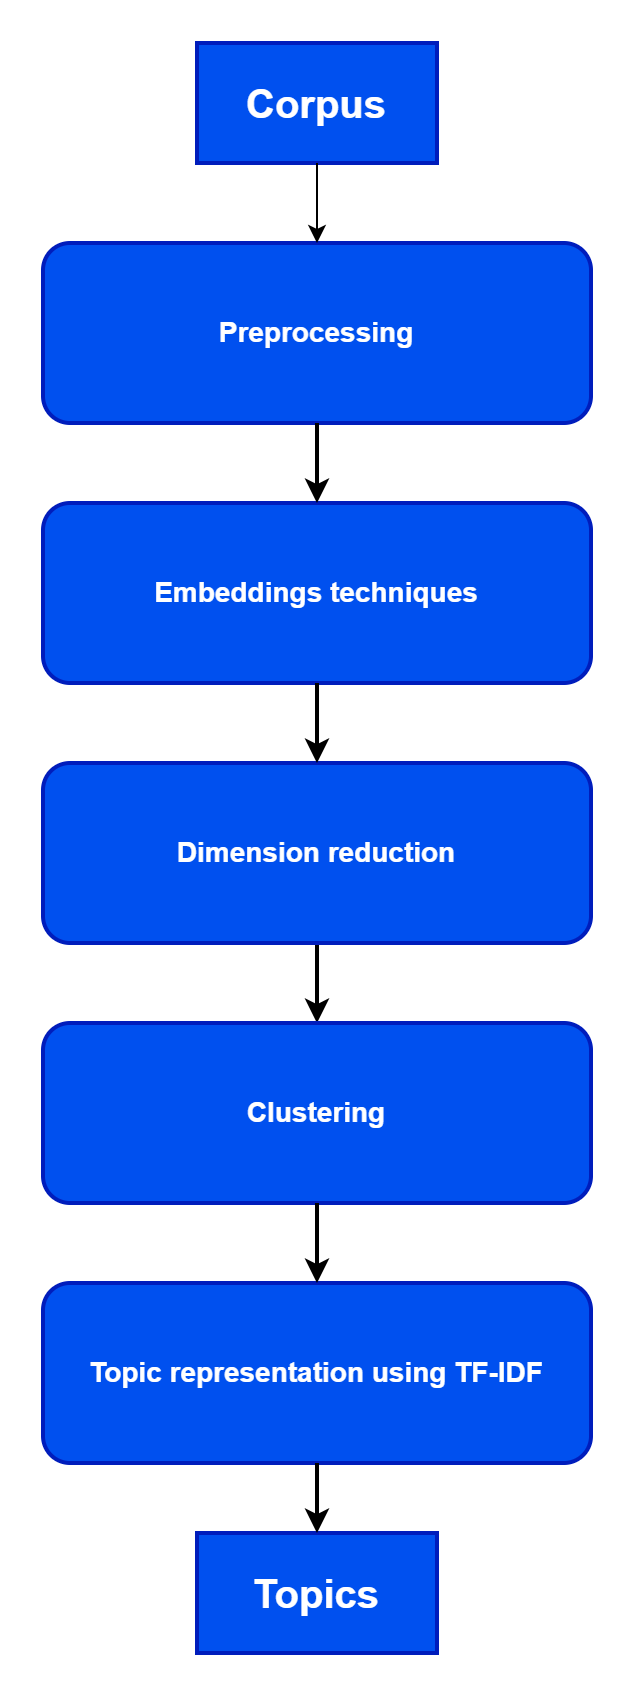
\includegraphics[width=0.4\textwidth]{images/describe_nlp.drawio.png}
    \caption{Algorithm description}
    \label{fig:nlp_describe}
\end{figure}

The process starts with preprocessing, which turns the given dataset into the form that is needed for the embedding techniques. Some soft clean is also applied to the corpus before translating the sentence into vectors. After we have the desired corpus, it will be represented as a vector in a fined vector space with the help of a sentence transformer. The dimension reduction techniques are then applied, and we use the output of the process as data points to do the main task of clustering. After that, we use a special version of TF-IDF to find the most significant word of each found topic.

\section{Preprocessing}

As you can see in the example of the raw database in section 7.3, The current data is stored in the Impala database. To begin to work with the data, I created a SQL script to pull the most recent transcription from the database and store it as a Pandas data frame, in the form of a pickle file. We will only need to pull the column that contains the value data.

\begin{table}[H]
\centering
\captionof{table}{Database description} \label{tab:description_database} 
\begin{tabular}{|lp{10cm}|lp{10cm}|}
\hline
\textbf{column name}  & \textbf{description}                                                                  \\ \hline
contact\_id           & ID of the conversation                                                                \\ \hline
transcript\_speaker   & 2 channels exist. Channel 1 is for our agent, and channel 2 is for the customer \\ \hline
transcript\_word      & Word of the transcript                                                                \\ \hline
transcript\_starttime & Time of each word when it is being spoken                                             \\ \hline
\end{tabular}
\end{table}

The data needs to be sorted in order. This is because when the words are being stored, it is not necessary in the order of the speaker. Only when we sort by transcript\_starttime and transcript\_speaker, we will have a correct order of the conversation. It is also important that the newest data is prioritized, which means when the data is selected, the partdate, which is the date that these pieces of information are recorded also needs to be sorted in ascending order.

After the data is in good order, The data is merged into conversations, with each row should have the same contact\_id. Here is the result of the process after the merge.

\begin{figure}[H]
    \centering
    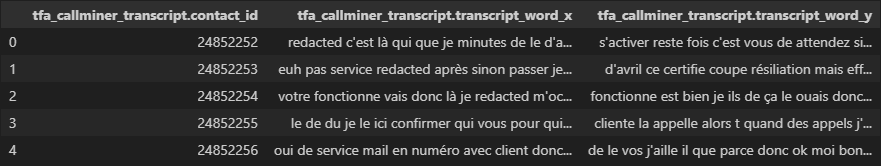
\includegraphics[width=1\textwidth]{images/dataset_merged_example.png}
    \caption{Dataset after the merge into big conversation}
    \label{fig:dataset_merge}
\end{figure}

It is not recommended to do the preprocessing with the corpus before feeding into a language model. However, the call here is a log of a speaking conversation. Speaking is not the same as writing, and we tend to put a lot of filler words to avoid emptiness while speaking. Therefore, before going to the next step of embedding the documents, These filler words should be removed to avoid confusion in the language model.

The French filler words vary, but 20\% of them can speak more than 90\% of the time. I only removed the word that I saw appear too many times.

\begin{lstlisting}[language=Python]
filler_word = ['redacted', 'bonjour', 'oui', 'monsieur', 'madame', 'ben', 'quelque', 'moment', 'justement', 'euh', 'non', 'hein', 'collègue', 'hein', 'allô', 'ah', 'alors', 'voilà', 'bah']
\end{lstlisting}

\section{Document embeddings}

We start by converting the current document that we just cleaned into numerical representation, and we will use a sentence transformer to do it.

A Sentence Transformer is a type of model designed to convert sentences or short text snippets into fixed-length vector representations, and we call it embeddings. These embeddings capture the semantic meaning and context of the input sentences, allowing for meaningful comparisons, similarity calculations, and downstream tasks in NLP.

Unlike traditional word embeddings, which generate vector representations for individual words, sentence transformers focus on creating embeddings for entire sentences. This is particularly useful when the meaning of a sentence is influenced by the arrangement and interaction of its words.

Sentence transformers are typically built using transformer architecture, which has proven highly effective in capturing contextual information and semantic relationships in text. The key innovation lies in how these models are fine-tuned to create sentence embeddings. During training, the model learns to generate embeddings in such a way that sentences with similar meanings are closer together in the embedding space, while sentences with different meanings are farther apart. Therefore, the application of clustering techniques for these embeddings is well-founded.

\subsection{CamemBERT}

Camembert is a state-of-the-art NLP model based on Roberta. It is part of the transformer-based architecture family, which has shown remarkable success in various NLP tasks. Camembert is specifically designed for understanding and generating human language text. It draws its name from the famous French cheese, just like the BERT model it is built upon.

Camembert is pre-trained on large amounts of text data to learn the underlying patterns and structures of language. This pre-training enables the model to understand the context, semantics, and relationships between words in a sentence. The key innovation of Camembert lies in its ability to understand sentences in French. Unlike Roberta that were trained in English, Camembert is trained in a French corpus.

In this case, we will use a specific version of CamemBERT, which is sentence transformer camemBERT. The model is Fine-tuned using pre-trained Facebook camembert-large and Siamese BERT-Networks with 'sentences-transformers' on dataset stsb.

\subsection{miniLMv2}

MiniLM is a compact and efficient language model developed by Microsoft Research. It's designed to offer a balance between model size and performance, making it well-suited for various natural language processing tasks. MiniLM is built upon the transformer architecture, which has proven to be highly effective for tasks like text generation, translation, and understanding.

One of the key features of MiniLM is its smaller size compared to its larger counterparts, such as BERT or RoBERTa. Despite its reduced size, MiniLM aims to retain competitive performance on a range of language-related tasks. This is achieved through careful optimization of the model architecture, training process, and compression techniques.

This architecture was updated in mid-2021 and has even better results and performance. In this project, a multilingual version of MiniLMv2 will be applied and we will have some comparison with CamemBERT. We will use the sentence transformer fine-tuned version of this model instead of the original one

\section{Dimension reduction}


\subsection{PCA}

Principal Component Analysis (PCA) is a traditional and widely used dimensionality reduction technique in the field of data analysis and machine learning. Its primary goal is to simplify the complexity of high-dimensional data while preserving as much relevant information as possible. PCA achieves this by transforming the original data into a new coordinate system where the dimensions, known as principal components, are orthogonal (uncorrelated) and capture the maximum variance in the data. 

Since the output of the sentence transformer still contains too many features, It is advised to use some techniques of dimensional reduction to reduce the number of features.

However, PCA still has some drawbacks:

\begin{itemize}
    \item Loss of Interpretability: The principal components are linear combinations of original features, which can make them difficult to interpret in terms of the original domain.
    \item Linearity Assumption: PCA assumes that the underlying relationships in the data are linear. It may not capture complex nonlinear patterns.
    \item Dependence on Variance: PCA focuses on variance, which might not be the most suitable criterion for all types of data or applications.
\end{itemize}


\subsection{UMAP}

UMAP (Uniform Manifold Approximation and Projection)\cite{mcinnes2020umap} is a powerful dimensional reduction method, high-dimensional data in a simpler, lower-dimensional space. It captures both global and local patterns, handles non-linearity, and adapts to the data's intrinsic structure. UMAP is stochastic, scalable, and useful for tasks like clustering and data exploration. It's available through open-source libraries and is widely used for various applications.

UMAP has been shown to be better than PCA in capturing nonlinear features, and also better in the task of finding topics in a corpus.



\section{Document clustering}

After reducing the number of dimensions, we will use its representation to clustering using several techniques.

\subsection{Kmeans}

K-means is the most widely used clustering algorithm in the field of unsupervised machine learning. Its primary objective is to partition a dataset into a predetermined number of distinct, non-overlapping clusters. K-means is particularly effective when the number of clusters is known or estimated, and it aims to minimize the variance within each cluster while maximizing the variance between clusters.

However, in our case, the number of clusters is unknown and it is hard to define the number of clusters. The good thing is that we don't need to find the exact big cluster, but also set multiple mini clusters and can extract the most important word out of these small topics. The output of the most important words of these small topics will be very close to each other and we can still suggest such important words for the end user.

\subsection{HDBSCAN}

HDBSCAN\cite{mcinnes2017hdbscan} (Hierarchical Density-Based Spatial Clustering of Applications with Noise) is a density-based clustering algorithm used for grouping data points that are close to each other in a high-dimensional space. Unlike traditional clustering methods that assume clusters to be of specific shapes and sizes, HDBSCAN is capable of identifying clusters of varying shapes and densities, making it particularly well-suited for complex and irregularly shaped clusters within noisy data. It is also an improved version of DBSCAN that detects automatically the number of clusters that need to be used instead of we need to define it. Therefore, it could be handy in our case since we don't know the exact number of topics that are needed.

\subsection{Hierachy clustering}

Agglomerative Clustering is a hierarchical clustering algorithm widely used for grouping data into clusters based on their similarity. Unlike partitioning algorithms like K-means, agglomerative clustering builds a hierarchy of clusters by iteratively merging or "agglomerating" data points or existing clusters. It starts with each data point as its own cluster and gradually combines them into larger clusters, forming a tree-like structure known as a dendrogram.

I will also apply this technique and compare it with HDBSCAN and Kmeans and we will compare the after all results.

\section{Topic representation using TF-IDF}

This is the most interesting part of this project. The TF-IDF used in this project is the modified version of TF-IDF but not the original one. SFR is an operator, a very specific environment with a dictionary of words that is used in the call is very technique and special. In every call that, the call center receives, there is a high chance that there are words that appear in every cluster (for example, telephone, signal, etc. ). With the documents level, these are important words, but we want to find something that is unique and only that cluster has. With this method, if the word appears in many other clusters, the ranking of the TF-IDF score will be lower.

\begin{figure}[H]
    \centering
    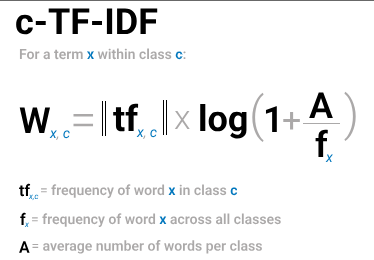
\includegraphics[width=0.4\textwidth]{images/tfidf.png}
    \caption{Modified version of TF IDF}
    \label{fig:tf-idf}
\end{figure}

This result would be importance scores for words within a cluster. The more important words are within a cluster, the more it is representative of that topic. In other words, if we extract the most important words per cluster, we get descriptions of topics.

Each cluster is converted to a single document instead of a set of documents. Then, we extract the frequency of word x in class c, where c refers to the cluster we created before. This results in our class-based tf representation. This representation is L1-normalized to account for the differences in topic sizes.

Then, we take the logarithm of one plus the average number of words per class A divided by the frequency of word x across all classes. We add plus one within the logarithm to force values to be positive. This results in our class-based idf representation. Like with the classic TF-IDF, we then multiply tf with idf to get the importance score per word in each class. In other words, the classical TF-IDF procedure is not used here but a modified version of the algorithm that allows for a much better representation.